\documentclass[12pt]{article}
\usepackage[margin=1in]{geometry}
\usepackage{amsmath}
\usepackage{amsfonts}
\usepackage{esint}
\usepackage{tikz-cd}
\usepackage{tikz}
\usepackage{graphicx}
\usepackage{hyperref}

\begin{document}

\title{Notes for B.C. Regan's Physics 17 Class, Fall 2022}
\author{Nathan Solomon}
\maketitle

\tableofcontents

\section{Week 1: Geometric Algebra}

\subsection{General rules}
Terminology: a $k$-blade is a multivector that can be written as the wedge product of $k$ vectors. A degree $k$ homogeneous multivector can be written as the sum of a bunch of $k$-blades. The rules below should work for any multivectors $a, b, c \in G(n, 0)$, although of course the rules that use the $\deg$ operator on a multivector also require that multivector to be homogeneous.
\begin{itemize}
    \item Associativity: $(ab)c = a(bc)$
    \item Left distributivity: $a(b+c) = ab+ac$
    \item Right distributivity: $(a+b)c = ac+bc$
    \item The dot product and wedge product are also both left and right distributive
    \item Scalar multiplication (let $\lambda$ be a scalar): $\lambda a = a \lambda = \lambda \cdot a = a \cdot \lambda = \lambda \wedge a = a \wedge \lambda$
    \item Dot product commutativity: $a \cdot b = b \cdot a$
    \item Wedge product anticommutativity: $a \wedge b = (-1)^{\deg(a) \deg(b)} b \wedge a$
    \item $\deg(a \cdot b) = | \deg(a) - \deg(b) |$
    \item $\deg(a \wedge b) = \deg(a) + \deg(b) \text{ if } \deg(a) + \deg(b) \leq n \text{ otherwise } a \wedge b = 0$
\end{itemize}

\subsection{Rules that might not work unless a and b are vectors}
\begin{itemize}
    \item Euclidean metric: $a^2 = ||a||^2$ where $||a||$ is a scalar
    \item $ab = a \cdot b + a \wedge b$
    \item $a \wedge b = - b \wedge a$
    \item $a \cdot b = \frac{1}{2}(ab + ba)$
    \item $a \wedge b = \frac{1}{2} (ab - ba)$
\end{itemize}

\subsection{Unit pseudoscalar}
Let $I \in G(n, 0) = e_1 \wedge e_2 \wedge \cdots \wedge e_n$. Then $I$ commutes with everything. If $n \in (4 \mathbb{Z} + \{0, 1\})$, we have the very nice property that $I^{-1} = I$, meaning that taking the dual of something twice has no net effect. If $n \in (4 \mathbb{Z} + \{2, 3\})$, we have the elegant-but-not-as-nice property that $I^{-1} = -I$, meaning that the unit pseudoscalar $I$ behaves like the imaginary unit $i = \sqrt{-1}$. Using geometric algebras in mischievous ways, we can coerce them into representing complex numbers, or even quaternions.

Reversing a list of $n$ unique elements by swapping adjacent elements requires $n(n-1)/2$ swaps (you can prove that with induction). That number of swaps is even if $n \equiv 0 \mod{4}$ or $n \equiv 1 \mod{4}$, and odd otherwise. Thus, the permutation that reverses $e_1 \wedge e_2 \wedge \cdots \wedge e_n$ is even if $n \in (4 \mathbb{Z} + \{0, 1\})$ and odd otherwise, which is why that property above works.

\subsection{Cross product \& wedge product}
The cross product of vectors exists only in $\mathbb{R}^3$, so the following properties work only in $G(3, 0)$.
\[I (a \times b) = a \wedge b\]
\[a \times b = -I (a \wedge b) = I (b \wedge a)\]


\subsection{Cool application of combinations}
The set of multivectors of degree $p$ in $\mathbb{F}^n$ has dimension ${n \choose p} = \frac{n!}{p!(n-p)!} $ over $\mathbb{F}$. Thus, the set of all multivectors in $\mathbb{F}^n$ has dimension $2^n$. For example, $G(3,0)$ (the set of multivectors in $\mathbb{R}^3$) has the basis $\{1, e_1, e_2, e_3, e_1 e_2, e_2 e_3, e_3 e_1, e_1 e_2 e_3\}$ over $\mathbb{R}$, which matches the 1-3-3-1 row from Pascal's triangle.

\section{Week 2: Microstates}

\subsection{Macrostates vs. microstates}
Suppose you have system of $N$ particles which each have a nonnegative integer amount of energy, and the total energy of the system is $E$, where $E \geq N$. Each way of distributing the energy between $N$ unordered particles is a macrostate, and each way of distributing the energy between $N$ ordered particles is a microstate. Counting microstates is useful because all microstate are equally likely, so we can figure out the probability that a particle will be at a given energy level. Counting macrostates is interesting but not really useful, and it's pretty difficult, because it requires a variation of the integer-partition-function.

Each microstate can be represented by a stars-and-bars diagram, where each star is a unit of energy. For example, in a system with $N=6$ and $E=8$, where one particle has energy=4, 2 particles have energy=2, and the rest have zero energy, the diagram could look like
\[\star \star \star \star | \star \star | \star \star | | |\]
But by convention, each partition in a stars-and-bars diagram must have at least one star, so we add one star to each partition by default, and instead write
\[\star \star \star \star \star | \star \star \star | \star \star \star | \star | \star | \star\]
The diagram below has the same distribution of energies but in a different order, meaning it represents the same macrostate, but a different microstate.
\[\star \star \star | \star \star \star \star \star | \star \star \star | \star | \star | \star\]
That microstate can be permuted $\frac{6!}{2!3!} = 60$ different ways, meaning that the corresponding macrostate contains 60 microstates. We could use factorial expressions like that to add up the total number of particles with energy $x$ across all microstates, but that would require a separate term for each macrostate, which would get very tedious. Instead, we'll find an explicit formula for that, which will only use one term.

\subsection{Nasty combinatorics stuff}
Define the function $\Omega$ as the total number of microstates accessible to our system.

\[\Omega(E, N) := \text{\# of microstates} = \sum_{\text{macrostates with $N$ particles \& energy $E$}} (\text{\# of permutations of that macrostate})\]

Going back to the first stars-and-bars diagram (the one where some partitions have zero stars), we have a total of $N+E-1$ characters: $E$ stars and $N-1$ bars. So the number of ways to arrange those characters is
\[\Omega(E, N) = {{N+E-1} \choose E} = {{N+E-1} \choose {N-1}} = \frac{(N+E-1)!}{E!(N-1)!} \]

In the example where $E=8$ and $N=6$, that tells us that there are $\Omega(8, 6) = 1287$ microstates.

\subsection{Deriving the discrete probability distribution}

Define the function
\[f(x, E, N) := \sum_{\text{microstates with $N$ particles \& total energy $E$}} (\text{\# of particles with energy $x$})\]

If we add up the number of particles in each microstate across all microstates, we get
\[\sum_{x=0}^E f(x, E, N) = N \cdot \Omega(x, E, N)\]

We can then expand $\Omega(x, E, N)$ using the Hockey Stick Identity:
\[\sum_{x=0}^E f(x, E, N) = N \cdot {{N+E-1} \choose {N-1}} = N \cdot \sum_{x=0}^E {{N+E-x-2} \choose {N-2}} \]

This leads to a very reasonable guess for what $f(x, E, N)$ is, which you can prove with induction if you take the base case to be $f(E,E,N) = N$.
\[f(x, E, N) = N \cdot {{N+E-x-2} \choose {N-2}}\]

Alternatively, you could prove that that works by using Pascal's identity plus induction, which is simpler but not as cool.

Now we can calculate the probability $p(x, E, N)$ that a random particle in our system will have energy $x$ (given that there are $N$ particles in the system, whose total energy is $E$). Note that the average number of particles in each microstate with energy $x$ is equal to $N$ times $p(x, E, N)$.
\[p(x, E, N) := \frac{f(x, E, N)}{N \Omega(E, N)} = \frac{(E+N-x-2)!}{(E-x)!(N-2)!} \cdot \frac{E!(N-1)!}{(N+E-1)!} = \frac{N-1}{E+N-1-x} \cdot \prod_{i=1}^x \frac{E+1-i}{E+N-i} \]

\section{Week 3: Thermodynamics}

\subsection{Laws of thermodynamics}
(taken from Wikipedia)

\textbf{0th Law:} If two systems are both in thermal equilibrium with a third system, then they are in thermal equilibrium with each other.

\textbf{1st Law:} In a closed system, $\Delta U_{system} = Q - W$ where $U$ is the total internal energy, $Q$ is the heat supplied to the system, and $W$ is the work done by the system (on its surroundings).

\textbf{2nd Law:} When two initially isolated systems in separate but nearby regions of space, each in thermodynamic equilibrium with itself but not necessarily with each other, are then allowed to interact, they will eventually reach a mutual thermodynamic equilibrium. The sum of the entropies of the initially isolated systems is less than or equal to the total entropy of the final combination. Equality occurs just when the two original systems have all their respective intensive variables (temperature, pressure) equal; then the final system also has the same values.

\textbf{3rd Law:} A system's entropy approaches a constant value as its temperature approaches absolute zero.

\subsection{Definitions of entropy \& temperature}
The entropy, $S$, of a system is defined in terms of the logarithm of the number of accessible microstates:
\[S := k_B \ln{\Omega(E)}\]
We can define temperature, $T$, in terms of the relationship between $E$ and $\Omega(E)$, if we pretend that $E$ and $\Omega(E)$ are differentiable.
\[\frac{1}{T} = \frac{\partial S}{\partial E} = \frac{k_B}{\Omega(E)} \cdot \frac{\partial \Omega(E)}{\partial E}\]
That simplifies to
\[T = \frac{\Omega(E)}{k_B \Omega'(E)}\]
This is a pretty unintuitive definition of temperature. One thing it does show clearly though is that for two systems that can exchange energy with each other, their total entropy is maximized when they are at the same temperature.

Since the definition of temperature is so wack, we often use the quantity $\beta$ instead.
\[\beta := \frac{1}{k_B T} \]
If we use the units electron-Volts and Kelvin, we can approximate room temperature as $300K$ (actual value is $293.15K$), and then $\beta$ at room temperature is roughly $40 (eV)^{-1}$ (actual value is $39.586 (eV)^{-1}$), since $k_B$ is $8.617 \times 10^{-5} eV/K$.

\subsection{Boltzmann factor}
Suppose you have a box of particles at thermal equilibirum which is split into two sides. The first one has energy $E_1$ and $\Omega(E_1)$ accessible microstates; the other has energy $E_2$ and $\Omega(E_2)$ accessible microstates. The two systems together have energy $E = E_1 + E_2$ and $\Omega(E)$ accessible microstates.

Assuming $E_2$ is small compared to $E_1$ and $E$, we can approximate $\ln \Omega(E_1)$ using the first order Taylor expansion of $\ln \Omega$, centered at $E$:
\[\ln \Omega(E_1) \approx \ln \Omega(E) - E_2 \left. \frac{\partial \ln \Omega(x)}{\partial x} \right|_{x=E}\]
where $x$ is a dummy variable. Using the definitions of entropy and temperature, that becomes
\begin{align*}
    \ln \Omega(E_1) &\approx \ln \Omega(E) - \frac{E_2}{k_B T} \\
    \frac{\Omega(E_1)}{\Omega(E)} &\approx \exp\Big( -\frac{E_2}{k_B T} \Big)
\end{align*}
If we suppose the second side of this system is a single particle, the approximation becomes essentially perfect.
\[\Omega(E_1) \propto e^{- E_2 / k_B T} \]
According to the \textbf{Fundamental Statistical Postulate (FSP)}, all microstates are equally likely, meaning the probability a particle will have energy $E_2$ is proportional to $\Omega(E_1)$.
\[P(E_2) \propto e^{- E_2 / k_B T} \]

\subsection{Derivation of Maxwell-Boltzmann velocity distribution}
The probability that a particle will have velocity $v = (v_x, v_y, v_z)$ is proportional to $e^{- \beta m v^2 / 2} dv$. That means we can define the probability distribution function as
\[F(v) dv = C e^{- \beta m v^2 / 2} dv\]
where $C$ is some constant. To determine what $C$ is, note that $F(v) dv$ integrated over all possible velocities is one, since probabilities always add to one.
\[\int_{v \in \mathbb{R}^3} F(v) dv = 1 \]
Now we just have to compute that integral.
\begin{align*}
    \int_{v \in \mathbb{R}^3} F(v) dv &= C \int_{\mathbb{R}^3} e^{- \beta m v^2 / 2} dv \\
    &= C \int_{\mathbb{R}} \int_{\mathbb{R}} \int_{\mathbb{R}} e^{- \beta m (v_x^2 + v_y^2 + v_z^2) / 2} dv_x dv_y dv_z \\
    &= C \Bigg( \int_{\mathbb{R}} e^{- \beta m v_x^2 / 2} dv_x \Bigg)^3 \\
    &= C \Bigg( \int_{\mathbb{R}} e^{- \beta m v_x^2 / 2} dv_x \Bigg)^3 \\
    &= C \Bigg( \int_{x \in \mathbb{R}} \int_{y \in \mathbb{R}} e^{- \beta m (x^2 + y^2) / 2} dx dy \Bigg)^{3/2} \\
    &= C \Bigg( \int_{r>0} \int_{\theta \in [0, 2\pi]} r e^{- \beta m r^2 / 2} d\theta dr \Bigg)^{3/2} \\
    &= C \Big( \frac{2 \pi}{\beta m} \Big)^{3/2} \\
    &= C \Big( \frac{2 \pi k_B T}{m} \Big)^{3/2}
\end{align*}
That means that
\[C = \Big( \frac{m}{2 \pi k_B T} \Big)^{3/2}\]
and
\[F(v) dv = \Big( \frac{m}{2 \pi k_B T} \Big)^{3/2} e^{-\frac{m v^2}{2 k_B T}} dv\]
But we don't want to know what velocities are likely; we care which speeds are likely. If we convert $v$ to spherical coordinates and integrate over infinitely thin spherical shells, we can calculate the probability distribution in terms of speed:
\[F(|v|) d|v| = 4 \pi v^2 \Big( \frac{m}{2 \pi k_B T} \Big)^{3/2} e^{-\frac{m v^2}{2 k_B T}} d|v|\]

\subsection{Equipartition theorem}
All particles in a system have the same RMS speed, and one way to show that is by finding an explicit formula for it.
\begin{align*}
    E_{avg} &= \int_{|v|=0}^\infty E \cdot F(|v|) d|v| \\
    &= \int_{|v|=0}^\infty \frac{m |v|^2}{2}  \cdot F(|v|) d|v| \\
    &= \int_{|v|=0}^\infty \frac{m |v|^2}{2} \cdot 4 \pi |v|^2 \Big( \frac{m}{2 \pi k_B T} \Big)^{3/2} e^{-\frac{m |v|^2}{2 k_B T}} d|v| \\
    &= \int_{v^2=0}^\infty \pi m v^3 \Big( \frac{m}{2 \pi k_B T} \Big)^{3/2} e^{-\frac{m v^2}{2 k_B T}} d(v^2) \\
    &= \pi m \Big( \frac{m}{2 \pi k_B T} \Big)^{3/2} \int_{x=0}^\infty x^{3/2} e^{-\frac{m x}{2 k_B T}} dx \\
\end{align*}
This is now a very painful integral, but it simplifies to
\[E_{avg} = \frac{3}{2} k_B T\]

From that equation, we infer that each degree of freedom has energy equal to
\[ \frac{k_B T}{2} \]


\subsection{Heat capacity}
Define the heat capacity, $C$, of a material as
\[C := \frac{\partial E_{avg}}{\partial T} \]

The heat capacity of an ideal gas that doesn't contain any vibration or rotational or chemical energy would be $1.5 k_B$, as shown above. The general rule is that the heat capacity of a material is the number of degrees of freedom per particle times $k_B / 2$. For example, in gases, there are 3 degrees of freedom: kinetic energy in each direction. For most metals, there are 6 degrees of freedom: 3 from kinetic energy in each direction and 3 from potential energy in each direction. For warm diatomic gases, there's the 3 degrees of freedom from kinetic energy plus two from rotational kinetic energy (rotating about the axis doesn't count since there's so little energy in that). For hot gases, there's those 5, plus 2 from the kinetic and potential energy from vibrating.

\subsection{Ideal gas law}
Consider an ideal gas moving in one dimension, with RMS speed $v_x$ along a line with length $L$, containing $N$ particles each of mass $m$. A particle moving at the RMS speed will collide with a wall with frequency $L / v_x$, and each time, it applies an impulse of $2 m v_x$. Therefore the average force each particle applies to the boundary of the line is $2 m v_x^2 / L$, and the total force on the boundary (averaged over time) is $F_x = 2 N m v_x^2 / L$. Note that $F_x$ is a scalar here. By making copies of that equation for the $y$ and $z$ directions and adding those 3 equations, we find that the total force (averaged over time) on the boundary of the box is
\[F= \frac{2Nmv^2}{L} \]
Since that equation is proportional to $v^2$, treating the gas as if all particles have speed equal to the RMS speed, as we did above, was indeed a valid move.

For our box, the volume is $V = L^3$ and the area of the walls is $A = 6L^2$. That means that the pressure the gas applies on the walls is
\[P = \frac{F}{A} = \frac{2Nmv^2}{6L^3} = \frac{Nmv^2}{3V} = \frac{2NE}{3V} \]
But we know a formula for average energy of the particles in an ideal gas is
\[E_{avg} = \frac{3 k_b T}{2}\]
Plugging in our formula for pressure and simplifying gives the ideal gas law:
\[P V = N k_B T\]

\section{Week 4: Bosons \& Fermions}

\subsection{Maxwell-Boltzmann distribution}
The Boltzmann factor $e^{-\beta E}$ that we've been using up till now is only an approximation for the actual energy distibutions of particles. The actual distribution function comes in two forms -- one for bosons and another for fermions. Bosons are particles with integers spin, and they follow Bose-Einstein statistics. Fermions are particles with half-odd-integer spin, and they follow Fermi-Dirac distributions.

These differ from the Maxwell-Boltzmann energy distribution because for both bosons and fermions, particles with the same energy are indistinguishable (although if the degeneracy is greater than one there may be other factors distinguishing the particles). This means that we need to count ``macrostates" instead of ``microstates" in order to calculate the discrete distribution functions. But for now, we just care about the continuous distribution functions.

Fermi-Dirac and Bose-Einstein statistics differ from each other because fermions have the additional restriction that each energy level (or sublevel, if degeneracy is greater than one) can only have one particle.

\subsection{Bose-Einstein distribution}
In Maxwell-Boltzmann statistics, particles are distinguishable, meaning all microstates are equally likely, but in Bose-Einstein statistics, particles are indistinguishable, so all macrostates are equally likely. So to understand the energy distribution of a bunch of bosons, instead of looking at the energy levels for individual particles, look at the occupancy of individual energy levels. For an energy level $E$, the energy is $nE$, where $n$ is the number of particles for the energy level, so the Boltzmann factor (assuming $E$ is fixed and $n$ is variable) is
\[e^{- \beta E n}\]
So the average occupancy of an energy level with energy $E$ is
\[\overline{n}(E) = \frac{\sum\limits_{N=0}^\infty N e^{- \beta E N}}{\sum\limits_{N=0}^\infty e^{- \beta E N}}\]
Now you can use the following Taylor series for a nifty trick:
\[\sum_{n=0}^\infty x^n = \frac{1}{1 - x} \]
Differentiate that and multiply by $x$ to get another identity:
\[\sum_{n=0}^\infty nx^n = \frac{x}{(1-x)^2} \]
Now let $x$ be $e^{-\beta E}$ and apply those two identities to the denominator and the numerator of the formula for $\overline{n}(E)$ to get
\[\overline{n}(E) = \frac{ \frac{x}{(1-x)^2} }{ \frac{1}{1-x} } = \frac{x}{1 - x} = \frac{e^{-\beta E}}{1 - e^{-\beta E}} = \frac{1}{e^{\beta E} - 1} \]
This derivation is not quite correct though -- we still need to multiply by the degeneracy, $g$, to account for multiple independent states with the same energy. Also, the derivation above used $e^{-\beta E}$ to represent the probability of a particle being in an energy level with energy level $E$ divided by the probability of a particle having energy $\mu$, where $\mu$ is the zero-point energy (energy of a particle in its ground state). Since $\mu$ might not be zero, the Boltzmann factor should be $e^{-\beta (E - \mu) N}$ instead of $e^{-\beta E N}$, so the correct formula for $\overline{n}$ is
\[\overline{n} = \frac{g}{e^{(E - \mu) \beta} - 1} \]

\subsection{Freeze-out}
If temperature is very large, we can approximate average energy of a bunch of bosons by replacing the exponent function with its linear approximation. To make this look nicer, we'll suppose $\mu$ is zero and $g$ is one.
\[E_\text{avg} = E \cdot \overline{n} = \frac{E}{e^{E / k_B T} - 1} \approx \frac{E}{(1 + E / k_B T) - 1} = k_B T\]

If you suppose each boson contibutes one degree of freedom, this is equivalent to the equipartition theorem. However, if temperature is very small, $E_\text{avg}$ (the energy of each harmonic oscillator) will be significally smaller than what we'd expect from the approximation above. This is especially true when $E - \mu$ is large (relative to $T$), as is the case for oscillating solid atoms of Beryllium, Boron, Carbon, or Silicon. According to the equipartition theorem, we'd expect the specific heat capacity of crystals to be around $3 k_B T = 25 J / \text{mol} K$, but because of freeze-out, it's actually a bit less, and for the atoms listed above with unusually stiff bonds, it's significantly less. On the other hand, there are also solids with molar heat capacity above $3 k_B T$, but that's due to other effects.

\subsection{Fermi-Dirac distribution}
After some practice drawing those funky energy-level diagrams we did in class, we clearly see that energy levels far below the Fermi energy $E_F$ are very likely to be completely full, and energy levels far above $E_F$ are very likely to be completely empty. To derive that, we can just calculate the average occupancy of each energy level as
\[\overline{n} (E) = \frac{\sum\limits_{N=0}^1 N e^{- \beta E N}}{\sum\limits_{N=0}^1 e^{- \beta E N}} \]
That's the exact same fomula we used to derive the Bose-Einstein distribution, except the possible values for occupancy of each energy level are just 0 and 1, instead of all nonnegative integers. Simply plugging in the values to the summations turns that formula into
\[\overline{n} = \frac{e^{- \beta E}}{1 + e^{- \beta E}} = \frac{1}{1 + e^{\beta E}} \]
But once again, we have to modify that to account for degeneracy of energy levels. We also have to account for the zero-point energy, but since occupied states are unavailable, we use the Fermi energy ($E_F$) instead, which is the highest energy of the states occupied at absolute zero.

So the correct formula for the average occupancy of each energy level according to Fermi-Dirac statistics is
\[\overline{n}(E) = \frac{g}{e^{(E - E_F) \beta} + 1} \]

\section{Week 5: Blackbody Radiation}

\subsection{Density of states in k-space}
For a standing harmonic wave in a one-dimensional container of length $L$, the ends must be nodes, so the wavevector $k$ can be any integer multiple of $\pi/L$. Each harmonic wave that satisfies the boundary conditions represents one possible state, so in $k$-space, the density of possible states is $L/\pi$. However, a standing sinusoidal wave with wavevector $k$ is exactly the same as a standing wave with wavevector $-k$, so to avoid counting the same state twice, we assume $k$ is positive. Now if you consider standing waves in a 3-dimensional box with volume $V$, and let $k$ be the 3D wavevector, then the density of states in $k$-space is $V/\pi^3$. That only applies to the quandrant where all 3 components of $k$ are positive, since the density of states is zero elsewhere. To make the next step easier, we can pretend the density of states in $k$-space is $(L/2\pi)^3$ everywhere. Then if we instead use $k$ to mean the wavenumber instead of the wavevector, then we can integrate over cencentric spherical shells in $k$-space to find that the density of states is
\[ dN = (4 \pi k^2 dk) \left( \frac{L}{2 \pi} \right)^3 = \frac{V k^2}{2 \pi^2} dk \]

But if we're these are light waves, there are two polarization states for each axis (this is sort of like the degeneracy of states), we double that to get
\[ dN = \frac{V k^2}{\pi^2} dk \]

Since we're considering photons, we can use the substitution $k = 2 \pi f / c$ where $f$ is temporal frequency. That also means that $dk = 2 \pi df / c$, so the density of states as a function of $f$ is
\[ dN = \frac{8 \pi V f^2}{c^3} df \]

\subsection{Spectral energy density}
The spectral energy density, $u(f, T)$ represents the energy per volume per frequency. That's equal to the energy per state, times the density of states, times the probability of being in each of those states, divided by the volume. Since the energy is $E = hf$, that works out to
\[E(f) \cdot N(f) \cdot \frac{1}{e^{E(f)/k_B T} - 1} \cdot \frac{1}{V} \]
Plugging in the formulas for $E$ and $N$, that becomes
\[u(f, T) = \frac{8 \pi h f^3}{c^3 (e^{hf/k_B T} - 1)} df\]
If you substitute in $f = c / \lambda$ and $df = - c d\lambda / \lambda^2$, you can also get the spectral energy density in terms of wavelength (although you also have to take the absolute value of that, since increasing $f$ means decreasing $\lambda$)
\[ u(\lambda, T) = - \frac{8 \pi h}{\lambda^3 (e^{h c / \lambda k_B T} - 1)} \Bigg( - \frac{c \, d\lambda}{\lambda^2} \Bigg) = \frac{8 \pi h c}{\lambda^5 (e^{h c / \lambda k_B T} - 1)} d\lambda \]
We also sometimes use the spectral radiance, $B$, instead of spectral energy density. Spectral radiance is the power emitted per unit area.
\[ B := \frac{c u}{4 \pi} \]

At large frequencies and small temperatures, you can approximate the Bose-Einstein distribution with the Maxwell-Boltzmann distribution:
\[ \lim_{f/T \rightarrow \infty} u(f, T) = \frac{8 \pi h f^3}{c^3} e^{-hf/k_B T} df \]
That approximation is called Wien's law, Wien's distribution law, or Wien's approximation. Don't confuse it with Wien's displacement law, which is described below. Similarly, you can come up with an estimation for small frequencies and large temperatures by using a first-order Maclauring series expansion of the Boltzmann factor:
\[ \lim_{T/f \rightarrow \infty} u(f, T) = \frac{8 \pi h f^3}{c^3 ((1 + hf/k_B T) - 1)} df  = \frac{8 \pi f^2 k_B T}{c^3} df \]
That equation is the classical approximation, called the Rayleigh-Jeans law. For a long time scientists were bamboozled by the ``ultraviolet catastrophe" -- the idea that according to this law, $u(f, T)$ should go to infinity as you look at higher and higher frequencies, which is clearly incorrect. This was solved by the correct formulas for $B$ and $u$ derived above, which are called Planck's law.

\subsection{Wien's displacement law}
Let $\lambda_{\text{max}}$ be the value of $\lambda$ such that $u(\lambda, T)$ is maximized. Note that $\lambda_\text{max}$ is a function of temperature. Wien's displacement law (different from Wien's law) states that $\lambda_\text{max} T$ is a universal constant.

You can also define $f_\text{max}$ to be the value of $f$ such that $u(f, T)$ is maximized. By the relation $\lambda = c / f$, that means $c T / f_\text{max}$ is also a constant, BUT NOT THE SAME CONSTANT. In fact, the latter is slightly larger.

\subsection{Stefan's law}
Imagine a hole in a box. The rate of effusion of particles is $A c / 4$, so the power emitted from that blackbody is
\begin{align*}
    P &= \frac{A c}{4} \int_0^\infty u(f, T) df \\
      &= \frac{A c}{4} \int_0^\infty \frac{8 \pi h f^3}{c^3 (e^{hf/k_B T} - 1)}  df \\
      &= \frac{2 \pi A h}{c^2} \int_0^\infty \frac{f^3}{e^{hf/k_B T} - 1} df \\
      &= \frac{2 \pi A h}{c^2} \Bigg( \frac{k_B T}{h} \Bigg)^4 \int_0^\infty \frac{x^3}{e^x - 1} dx \\
      &= \frac{2 \pi k_B^4 T^4 A}{c^2 h^3} \int_0^\infty \frac{x^3}{e^x - 1} dx
\end{align*}
That funky integral is difficult to evaluate. Lucikly online resources have figured out how to do it for us.
\begin{align*}
    \int_0^\infty \frac{x^3}{e^x - 1} dx &= \int_0^\infty \frac{x^3 e^{-x}}{1 - e^{-x}} dx \\
    &= \int_0^\infty x^3 e^{-x} \sum_{n=0}^\infty (e^{-x})^n dx \\
    &= \int_0^\infty x^3 \sum_{n=1}^\infty e^{-nx} dx \\
    &= \sum_{n=1}^\infty \int_0^\infty x^3 e^{-nx} dx \\
    &= \sum_{n=1}^\infty \int_0^\infty \left( \frac{y}{n} \right)^3 e^{-y} \left( \frac{dy}{n} \right) \\
    &= \sum_{n=1}^\infty \frac{1}{n^4} \cdot \int_0^\infty y^3 e^{-y} dy \\
    &= \zeta(4) \cdot \Gamma(4) \\
    &= \frac{\pi^4}{90} \cdot (3!) \\
    &= \frac{\pi^4}{15}
\end{align*}
Therefore we can solve for the ``blackbody radiant emittance" ($j^\star = P / A$):
\[ j^\star = \sigma T^4 \]
That equation is Stefan's law, and $\sigma$ is the Stefan-Boltzmann constant.
\[ \sigma := \frac{2 \pi^5 k_B^4}{15 c^2 h^3} \]
That works only for blackbodies though -- if we want to generalize it to work for other materials, we can say
\[ j^\star = a \sigma T^4 \]
Where $a$ is the absorptivity/emissivity of the material (which is 1 for blackbodies, and somewhere between 0 and 1 for other materials).

\subsection{Debye sphere}
Stefan's law doesn't have a clear intuitive interpretation, but here's one way to think about it. Suppose you're in $k$-space, and have a sphere of radius $k_D$ that encloses pretty much all of the occupied $k$-states. According to the equipartition theorem, energy is proportional to $k_B T$, so energy per $k$-state is proportional to $T$. But according to the Planck relation and the equipartition theorem, the energy corresponding to a photon with wavenumber $k_D$ is
\[ E = h c k_D / 2 \pi = k_B T \]
which means as $T$ increases, the radius of the Debye sphere must increase proportionally to $T$, which means the number of occupied states enclosed by the sphere increases cubically with $T$. Since power is proportional to the number of states and also to the energy per state, it will increase quartically with temperature.

\section{Week 6: Bohr \& Rutherford}

This week's notes is a whole hodgepodge of experiments and new ideas from the early 1900s.

\subsection{Miscellaneuous Experiments (in no particular order)}
\begin{itemize}
    \item J.J. Thomson figures out that cathode rays are made of electrons
    \item Thomson measures charge-to-mass ratio of electron by using a velocity selector
    \item Fletcher \& Millikan's oil drop experiment determines the quantized unit of electric charge
    \item Michael Faraday discovers his law of electrolysis
    \item Rutherford shows that positive charge is concentrated at tiny centers of atoms
    \item Kirchhoff realizes that the emissivity and the absorptivity of a material are the same. He also explains Fraunhofer D-lines.
    \item Bunsen uses absorption spectra of the sun to show what elements are present on its surface
    \item Balmer comes up with experimental formula for wavelengths of emission lines of hydrogen
    \item Bohr proposes electrons orbit in ``stationary states", which don't follow classical rules for Bremsstrahlung
    \item Franck \& Hertz show that when electrons are fired through mercury vapor, the amount of energy they lose can only be an integer multiple of 4.9 eV, which confirms Bohr's atomic model
\end{itemize}

\subsection{Bohr's Model}
Bohr proposed that the orbital angular momentum of an electron can only be an integer multiple of the reduced Planck constant:
\[ L := m_e v r \in \hbar \mathbb{N} \]
In the Bohr model, whenever an atom absorbs or emits a photon, the frequency of that photon is unrelated to the frequency of the electron's orbit, which makes no sense if you think of it in terms of classical physics.

For a hydrogen atom, the centripetal force on an electron is
\[ F = \frac{m_e v^2}{r} = \frac{ke^2}{r^2} \]
where $k := 1 / (4 \pi \varepsilon_0)$. From that, you can use more classical physics to get the potential energy ($U$), kinetic energy ($K$), and total energy ($E$) of the electron.
\[ U =  - \frac{k e^2}{r} , K = \frac{k e^2}{2 r} , E = - \frac{k e^2}{2 r} \]
You can now solve for the velocity:
\[ v = r^2 F / L = \frac{k e^2}{n \hbar} \hspace{1cm} \forall n \in \mathbb{N}\]
And the radius:
\[ r = \frac{n \hbar}{m_e v} = \frac{n^2 \hbar^2}{m_e k e^2} \hspace{1cm} \forall n \in \mathbb{N} \]
That quantity when $n=1$ is called the Bohr radius, $a_0$
\[ a_0 := \frac{\hbar^2}{m_e k e^2} = \frac{h^2 \varepsilon_0}{\pi m_e e^2} \approx .5292 \text{\AA} \]

\subsection{Rutherford Scattering}
If you fire a beam of $\alpha$ particles at a perpendicular sheet of gold foil, you might expect them to go right through, and most do, but some will be scattered. The number of particles you'll detect that are scattered at an angle $\phi$ is
\[ \Delta n = \frac{k^2 Z^2 e^4 N n A}{4 R^2 E^2 \sin^4 (\phi / 2)} \]
where $k$ is Coulomb's constant, $Z$ is the atomic number of the metal, $N$ is the number of nuclei per unit area, $n$ is the number of $\alpha$ particles scattered per unit time, $A$ is the area of the detector, $R$ is the distance from the detector to the point where $\alpha$ particles hit the foil, and $E$ is the kinetic energy of each $\alpha$ particle.

We do not need to know the derivation of that formula, only that it comes from electrostatic repulsions between the metal nuclei and the $\alpha$ particles. If the $\alpha$ particles are moving fast enough, they will actually touch the surface of the nuclei, and that equation will stop working.

\subsection{Compton Scattering}
To make this derivation extra fun, we'll use 4-momentum. Normally that means using the Minkowski product, but I don't like that -- I prefer to just make the time component of 4-momentum imaginary, which has the same effect as using a (-1, 1, 1, 1) metric signature.
\[ \boldsymbol{p} := \begin{bmatrix}
    iE/c \\
    p_x \\
    p_y \\
    p_z
\end{bmatrix} \]
This works out nice because $\boldsymbol{p}^2 = p^2 - E^2/c^2 = p^2 - (p^2 c^2 + m_0^2 c^4) / c^2 = - m_0^2 c^2$ which means that $\boldsymbol{p}$ is Lorentz invariant.

Compton scattering describes a photon colliding with an electron. Suppose the  electrons starts at rest, and a photon is moving right (in the +x direction towards it). After colliding, the electron is moving up and to the right, at an angle $\theta$ above the horizontal, and the photon is moving down and to the right, at an angle $\phi$ below the horizontal. We want to be able to find how much the wavelength of the photon changes, given the angle $\theta$.

\begin{figure}[h]
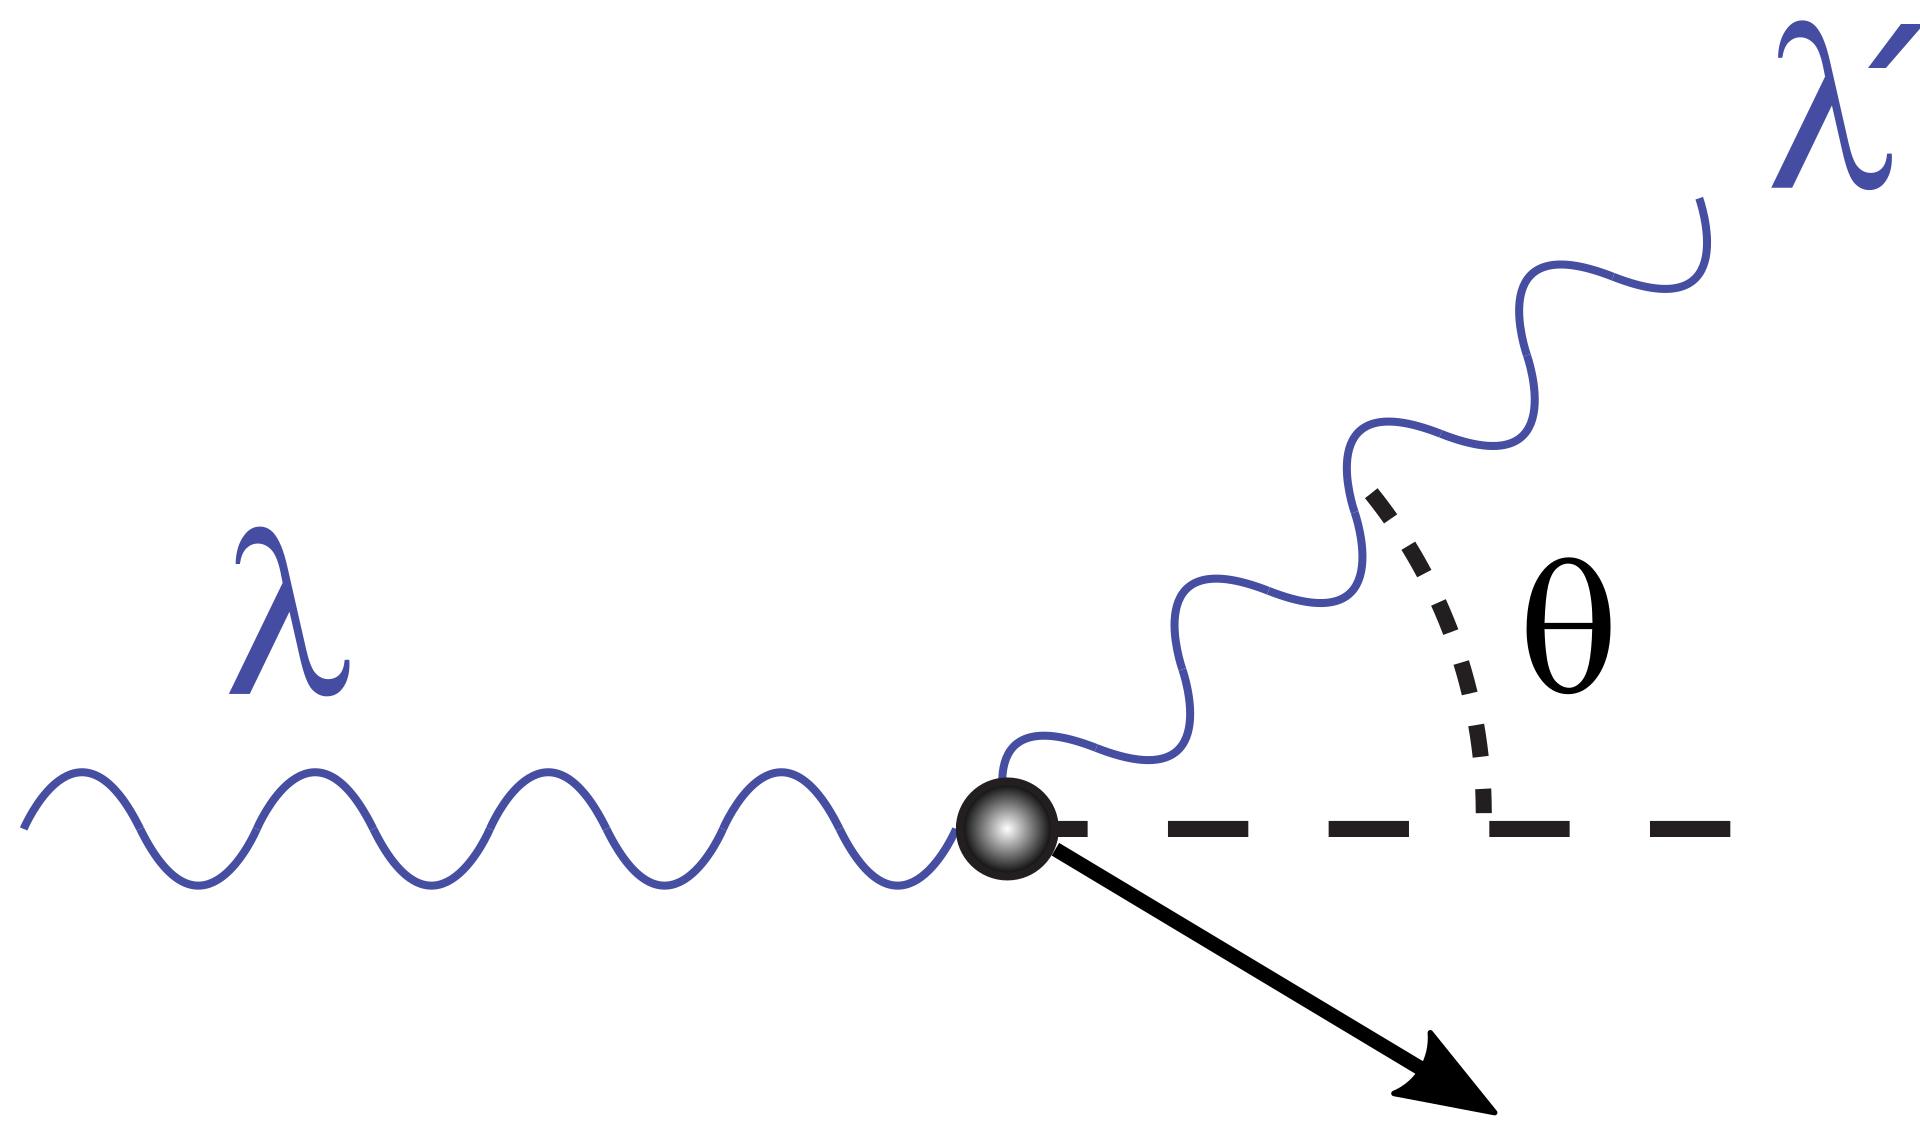
\includegraphics[width=8cm]{Compton-scattering.png}
\centering

By JabberWok, CC BY-SA 3.0, \url{https://commons.wikimedia.org/w/index.php?curid=2078004}
\end{figure}
Now we can use the conservation of 4-momentum to solve for $\lambda' - \lambda$
\[ \boldsymbol{p_\gamma} + \boldsymbol{p_e} = \boldsymbol{p_\gamma '} + \boldsymbol{p_e '} \]
Next, substitute in the definition of 4-momentum, and the fomulas for momentum and energy of a photon
\[ \begin{bmatrix} i h / \lambda \\ h / \lambda \\ 0 \\ 0 \end{bmatrix}
+ \begin{bmatrix} i m_e c \\ 0 \\ 0 \\ 0 \end{bmatrix}
= \begin{bmatrix} i h / \lambda' \\ (h / \lambda') \cos \theta \\ (h / \lambda') \sin \theta \\ 0 \end{bmatrix}
+ \boldsymbol{p_e '} \]
Since the electron does not gain or lose mass, the norm of its 4-momentum doesn't change, so
\[ \left( \begin{bmatrix} i h / \lambda \\ h / \lambda \\ 0 \\ 0 \end{bmatrix}
+ \begin{bmatrix} i m_e c \\ 0 \\ 0 \\ 0 \end{bmatrix}
- \begin{bmatrix} i h / \lambda' \\ (h / \lambda') \cos \theta \\ (h / \lambda') \sin \theta \\ 0 \end{bmatrix} \right)^2
= (\boldsymbol{p_e'})^2 = (\boldsymbol{p_e})^2 = - m_e^2 c^2 \]
The left hand side of that equation simplifies to
\begin{align*}
    - m_e^2 c^2 &= \begin{bmatrix} i h / \lambda + i m_e c - i h / \lambda' \\ h / \lambda - (h / \lambda') \cos \theta \\ - (h / \lambda') \sin \theta \\ 0 \end{bmatrix}^2 \\
                &= (ih/\lambda + im_ec - ih/\lambda')^2 + (h/\lambda - h\cos \theta / \lambda')^2 + (-h \sin \theta / \lambda')^2 \\
                &= - m_e^2c^2 - 2hm_ec/\lambda + 2h^2/(\lambda' \lambda) + 2hm_ec/\lambda' - 2h^2\cos \theta / (\lambda' \lambda)
\end{align*}
Now all you have to do is manipulate that equation a bit more
\begin{align*}
    - m_e^2 c^2 &= - m_e^2c^2 - 2hm_ec/\lambda + 2h^2/(\lambda' \lambda) + 2hm_ec/\lambda' - 2h^2\cos \theta / (\lambda' \lambda) \\
    0 &= - 2m_ec/\lambda + 2h/(\lambda' \lambda) + 2m_ec/\lambda' - 2h\cos \theta / (\lambda' \lambda) \\
    0 &= -m_ec\lambda' + h + m_ec\lambda - h\cos \theta \\
    \lambda' - \lambda &= \frac{h}{m_e c} (1 - \cos \theta) = \lambda_C (1 - \cos \theta)
\end{align*}
That last equation is the formula for Compton scattering. The Compton wavelength of a particle with mass $m$ is a useful constant, defined as $\lambda_C := h/(m c)$.

\section{Week 7: Matter Waves}

\subsection{Cool Integral Trick}
Before starting the actual notes, here's a fun integral. It's particularly useful for solving all those problems where you average something over a probability distribution. It assumes $\operatorname{Re}(a)>0$ and $n \in \mathbb{N}$.
\begin{align*}
    \int_0^\infty x^n e^{-x/a} dx &= \int_0^\infty (a^n y^n) e^{-y} (a \, dy) \\
    &= a^{n+1} \int_0^\infty y^n e^{-y} dy \\
    &= a^{n+1} \Gamma(n+1) \\
    &= n! \, a^{n+1}
\end{align*}

\subsection{Another Unrelated Topic}
We should memorize this definition of the fine-structure constant:
\[ \alpha := \frac{e^2}{4 \pi \varepsilon_0 \hbar c} = \frac{e^2}{2 \varepsilon_0 h c} \approx \frac{1}{137} \]
It was also recommended that we remember the following approximations:
\[ \hbar c \approx 197 \text{ eV nm} \]
\[ \frac{e^2}{4 \pi \varepsilon_0} \approx 1.44 \text{ eV nm} \]

\subsection{Dispersion Relations}
This is pretty much all we need to know about dispersion relations (for now):
\[ v_\text{phase} = \omega / k \]
\[ v_\text{group} = \frac{\partial \omega}{\partial k} \]
For all matter waves, the geometric mean of the phase velocity and the group velocity is $c$, the speed of light. For non-dispersive waves, such as light traveling through a vacuum, the phase and group velocities are both $c$.

\subsection{Uncertainty Principle}
Suppose you have some signal, which is a function of time, and you measure $n$ samples from it, which are evenly spaced time $\Delta t$ apart. Now you know that that signal exists within a window of time with width $\sigma_t := n \Delta t$, so that represents your ``uncertainty in time". But suppose you also want to measure the frequency of the signal. According to the Nyquist-Shannon sampling theorem, the highest frequency you can extract from your samples is $1/(2 \Delta t)$. Trying to measure the frequencies that exist in the signal is equivalent to trying to reconstruct the signal using the sum of several sinusoids, and in this case, you need $n$ sinusoids whose frequencies are evenly spaced, ranging from zero to $1/(2\Delta t)$ (including the upper bound, but not including zero). That means the lowest frequency you can measure using the $n$ samples is $\sigma_f := 1/(2n\Delta t)$, which represents your ``uncertainty in frequency". This allows you to write the uncertainty principle, which is true no matter what you choose $n$ and $\Delta t$ to be.
\[ \sigma_t \sigma_f \geq \frac{1}{2} \]
However, if you define $\sigma$ to be the standard deviation of a function, instead of the width of the window where the function is non-zero, then you can get an even smaller bound. In next week's notes, we'll see how to minimize that bound and do a whole bunch of other cool stuff with that.

\subsection{Fourier Inversion Theorem}
The inverse Fourier transform of the Fourier transform of $f(x)$ is
\begin{align*}
    \mathcal{F}^{-1}(\mathcal{F}(f))(x) &= \frac{1}{\sqrt{2 \pi}} \int_{-\infty}^\infty \left( \frac{1}{\sqrt{2 \pi}} \int_{-\infty}^\infty f(x') e^{-ikx} dx' \right) e^{ikx} dk \\
    &= \int_{-\infty}^\infty f(x') \left( \frac{1}{2 \pi} \int_{-\infty}^\infty e^{-ik(x - x')} dk \right) dx' \\
    &= \int_{-\infty}^\infty f(x') \delta(x - x') dx' \\
    &= f(x)
\end{align*}
This proves that $\mathcal{F}^{-1}$ and $\mathcal{F}$, as we have defined them, are indeed inverses, which is good. That proof above uses the Dirac $\delta$ ``function", which is more like the limit of a function than an actual function, but it makes everything work out nicely, so we leave out the nitty-gritty details.

\section{Week 8: Fourier Stuff}

\subsection{Angular Frequency Fourier Transform}
The formula you'll typically find online for the Fourier transform (and it's inverse) convert between time domain and frequency domain, but since we often want to think in terms of angular frequency instead of frequency, we use these definitions.
\begin{align*}
    (\mathcal{F} f)(k) &:= \frac{1}{\sqrt{2 \pi}} \int_{x \in \mathbb{R}} f(x) e^{-ikx} dx \\
    (\mathcal{F}^{-1} g)(x) &:= \frac{1}{\sqrt{2 \pi}} \int_{k \in \mathbb{R}} g(k) e^{ikx} dk
\end{align*}
In my opinion, this is still is a strange way to write it -- if it were up to me, I'd replace the $1/\sqrt{2 \pi}$ in the first equation with $1/2 \pi$ and remove the $1/\sqrt{2 \pi}$ in the second equation. However, this is how the textbook and lecture notes chose to write them, and it's still valid, so we will use those definitions throughout the class.

\subsection{Common Fourier Transforms}
There are three conversions we need to know. (1) The Fourier transform turns a Gaussian function into another Gaussian, (2) it turns $\operatorname{rect}$ into $\operatorname{sinc}$ (and vice versa), which can be used to explain diffraction gratings, and (3) it turns a constant function into the Dirac $\delta$ ``function".

\subsection{Properties of Fourier Transforms}
If $f$ and $g$ are functions, define their convolution as
\[ (f * g)(t) := \int_{-\infty}^\infty f(\tau)g(t-\tau)d\tau \]
This has lots of cool properties, notably that $f * \delta = f$ if $f$ is a nice, smooth function. For Fourier transforms, we have the following properties:
\begin{itemize}
    \item $\mathcal{F}(f * g) = \sqrt{2 \pi} \cdot (\mathcal{F} f) \cdot (\mathcal{F} g)$ (the constant is only there cuz we're using a weird version of $\mathcal{F}$
    \item $(\mathcal{F} f^{(n)}) (\omega) = (i \omega)^n (\mathcal{F} f)(\omega)$ where $f^{(n)}$ is the $n$th derivative of $f$.
\end{itemize}
It's also good to know what happens to the frequency domain of a signal when you shift or scale the time domain signal. And of course, it's good to know how to apply all those properties in reverse as well.

\subsection{Uncertainty Principles}
The fuzzier (wider) a signal is in the time domain, the sharper (skinnier) it will be in the frequency domain, and vice-versa. The product of those uncertainties is minimized when the signal is a Gaussian (idk how to prove that), in that case, we get the lower limit, $\Delta x \Delta k = \frac{1}{2}$. In general, we have the following relations:
\begin{align*}
    \Delta x \Delta k &\geq \frac{1}{2} \\
    \Delta t \Delta \omega &\geq \frac{1}{2} \\
    \Delta x \Delta p &\geq \frac{\hbar}{2} \\
    \Delta t \Delta E &\geq \frac{\hbar}{2}
\end{align*}

\section{Week 9: Wave Function}

\subsection{Time-Independent Schrödinger Equation}
This only works for steady states, where the wave function does not change over time. In these cases, the total energy $E$ is the eigenvalue of the Hamiltonian operator, $H := i \hbar \frac{\partial}{\partial t}$, (on $\psi$).
\[ - \frac{\hbar^2}{2m} \cdot \frac{d^2}{dx^2} \psi(x) + U(x) \cdot \psi(x) = E \cdot \psi(x) \]
This works because we can define $k := -i \hbar \frac{d}{dx}$ as an operator, so the terms on the left hand side of that equation can be thought of as representing kinetic and potential energy, respectively.

\subsection{Particle in a Box}
A free particle is not bound, therefore not quantized. However, if a particle is trapped in a one dimensional box of length $L$, its wavefunction is
\[ \psi(x) = \sqrt{ \frac{2}{L} } \cdot \sin \left( \frac{\pi n x}{L} \right) \]
Since a free particle has energy $E = \hbar^2 k^2 / 2m$, and this bound particle has $k = \pi n / L$, its energy is
\[ E = \frac{\hbar^2 \pi^2 n^2}{2 m L^2} \]

\subsection{Harmonic Oscillator}
Consider a mass on a spring, whose natural angular frequency is $\omega_0$. In the ground state ($n=0$), the wavefunction and the probability distribution are both perfect Gaussians.
\[ \psi_0 = \left( \frac{\omega_0 m}{\pi \hbar} \right)^{1/4} e^{- \omega_0 m x^2 / (2 \hbar)} \]
In general, the $n$th excited state for a quantum harmonic oscillator will have $n$ nodes, and a total energy of $E= \hbar \omega_0 (n + \frac{1}{2})$.

Since energy is, on average, shared evenly between kinetic and potential, and since the average position and momentum of the oscillator are both zero, you can use the properties of variance to show that for a harmonic oscillator in the $n$th excited state,
\[ \Delta x \Delta p = \hbar (n + \frac{1}{2}) \]
Looking at it this way explains why zero-point energy has to be a thing -- if a quantum harmonic oscillator had any less energy than the zero-point energy, it would violate the Heisenberg uncertainty principle.

\subsection{Useful Integral}
Because we have to work with Gaussians so much now, it's good to know this formula (you can also halve it to get the integral from zero to $\infty$, instead of from $-\infty$ to $\infty$, since it's symmetric):
\[ \int_{-\infty}^\infty x^2 e^{-ax^2} dx = \frac{1}{2a} \sqrt{ \frac{\pi}{a} } \]
Of course, that is mean to work only when $a$ is positive.

\subsection{Tunneling}
If a stream of particles with kinetic energy $E$ has a wavefunction with amplitude $A$ and wavenumber $k$, and it is incident on a potential barrier of finite width (that is, potential energy is zero when $x<0$ and $U$ when $x>0$), and we define $\alpha = 1/\delta = \frac{1}{\hbar} \sqrt{2m(U-E)}$, where $\delta$ is the penetration depth, then we can figure out the reflection and transmission coefficients, $R$ and $T$, as well as the amplitude of the wavefunction of the transmitted wave, which we call $B$, using this formula:
\[ R = 1 - T = \left| \frac{B}{A} \right|^2 = \left| - \frac{1 + ik / \alpha}{1 - ik / \alpha} \right|^2 \]
Note that if $U<E$ then $\alpha$ will be imaginary instead of real, so there will be a transmitted wave, instead of decaying exponentiall when $x>0$.

\section{Week 10: Review}

\subsection{Notecard for midterms \& final}
This section has all of the most important equations to include on your notecard EXCEPT for the stuff that was in notes from previous weeks (e.g. the Maxwell-Boltzmann speed distribution, the blackbody radiation equation, et cetera).

\subsection{Virial Theorem}
For a system in which the potential energy due to each pair of particles is proportional to $r^n$, where $r$ is the distance between the particles and $n$ is an integer, the total kinetic energy (averaged over a long time) of the system is $n/2$ times the potential energy (averaged over a long time) of the system. Notably, $n=2$ for a harmonic oscillator, and $n=-1$ for a gravitational system or a hydrogen atom.

We can use this to find that for a giant cloud of $N$ gas particles dominated by gravitational force, the specific heat is
\[ C = - \frac{3}{2} N k_B \]

\subsection{Lorentz Invariants}
Define the following 4-vectors (with the weird Minkowski metric, unless you prefer to multiply the first component of each by $i$):
\begin{align*}
    \boldsymbol{r} &= (ct, x, y, z) \\
    \boldsymbol{k} &= (\omega/c, k_x, k_y, k_z)
\end{align*}
Then $s := |\boldsymbol{r}|$ and $\phi := \boldsymbol{k} \cdot \boldsymbol{r}$ and $|\boldsymbol{k}|$ are invariants.

\subsection{Partition function}
\[ Z := \sum_i g_i e^{-\beta E_i} = \int g e^{- \beta E} dE \]
\[E_{avg} = \frac{\sum_i E_i e^{-\beta E_i}}{\sum_i e^{-\beta E_i}} = \frac{\int E e^{-\beta E} dE}{\int e^{-\beta E} dE}  = - \frac{\partial}{\partial \beta} \ln Z\]

\subsection{Spherical coords}
\begin{align*}
    x &= r \sin \theta \cos \phi \\
    y &= r \sin \theta \sin \phi \\
    z &= r \cos \theta \\
    dx \, dy \, dz &= r^2 \sin \theta \, dr \, d\theta \, d\phi
\end{align*}

\subsection{Summation identities}
The following Taylor series converges on $x \in (-1, 1)$.
\[\sum_{n=0}^\infty x^n = \frac{1}{1-x} \]
Differentiate that and multiply by $x$ to get this formula:
\[\sum_{n=0}^\infty nx^n = \frac{x}{(1-x)^2} \]

\subsection{Binomial coefficients}
\[ \binom{n}{k} := \frac{n!}{k! (n-k)!} \]
Pascal's identity:
\[\binom{n}{k} = \binom{n-1}{k} + \binom{n-1}{k-1}\]
Binomial theorem:
\[(a+b)^n = \sum_{k=0}^n \binom{n}{k} a^k b^{n-k}\]

\subsection{Energy-momentum equation}
In general, I'll use $m$ to denote the rest mass, and $\gamma m$ to mean the relativistic mass.
\[E^2 = m^2 c^4 + p^2 c^2\]
In that equation, $E$ is the kinetic energy plus the rest energy. The momentum is $p = \gamma m v$, and the rest energy is $mc^2$, so the kinetic energy must be
\begin{align*}
    K &= E - mc^2 \\
      &= \sqrt{m^2 c^4 + p^2 c^2} - mc^2 \\
      &= \sqrt{m^2 c^4 + \frac{m^2 v^2 c^2}{1 - \frac{v^2}{c^2}}} - mc^2 \\
      &= m c \sqrt{\frac{(c^2 - v^2) + v^2}{1 - \frac{v^2}{c^2}}} - mc^2 \\
      &= m c^2 \left( \sqrt{\frac{1}{1 - \frac{v^2}{c^2}}} - 1 \right) \\
      &= (\gamma - 1) m c^2
\end{align*}
This makes sense, because then the total energy is $E = \gamma m c^2$.

\subsection{Maxwell's equations}
Let $D := \varepsilon_0 E + P$ where $P$ is the polarization field, and let $H := \frac{B}{\mu_0} - M$ where $M$ is the magnetization field. Then the following version of Maxwell's equations work even if you aren't in a vacuum:
\begin{align*}
    \nabla \cdot D &= \rho \\
    \nabla \cdot B &= 0 \\
    \nabla \times E &= - \frac{\partial B}{\partial t} \\
    \nabla \times H &= J + \frac{\partial D}{\partial t}
\end{align*}
If you're in a vacuum, you can use the identity $\nabla \times (\nabla \times E) = \nabla (\nabla \cdot E) - \nabla^2 E$ to derive the 3D wave equation for electromagnetic waves:
\[ \nabla^2 E = \frac{1}{c^2} \cdot \frac{\partial^2 E}{\partial t^2} \]

\subsection{Maxwell-Boltzmann speed distribution}
\begin{align*}
    \text{probability density} &= 4 \pi v^2 \Big( \frac{m}{2 \pi k_B T} \Big)^{3/2} e^{-\frac{m v^2}{2 k_B T}} dv \\
                               &= 2 \sqrt{E/\pi} \Big( \frac{1}{k_B T} \Big)^{3/2} e^{-E / k_B T} dE
\end{align*}

\begin{tabular}{ c|c|c } 
    & Speed & Energy \\
    \hline
    Mean & $\sqrt{ \frac{8kT}{\pi m} }$ & $ \frac{3}{2} kT$ \\ 
    \hline
    RMS & $\sqrt{ \frac{3kT}{m} }$ & $ \frac{\sqrt{15}}{2} kT$ \\ 
    \hline
    Mode & $\sqrt{ \frac{2kT}{m} }$ & $\frac{kT}{2}$ \\ 
\end{tabular}

\subsection{Wien's law}
\[ \lambda_\text{max} T(\lambda_\text{max}) = 2.898 \times 10^{-3} mK \]

\subsection{Angular frequency version of Fourier transform}
If $f$ is a function of $x$:
\[ (\mathcal{F}f)(k) = \frac{1}{\sqrt{2 \pi}} \int_{-\infty}^\infty e^{-ikx}f(x) dx \]
If $f$ is a function of $k$:
\[ (\mathcal{F}^{-1}f)(x) = \frac{1}{\sqrt{2 \pi}} \int_{-\infty}^\infty e^{ikx}f(k) dk \]

\subsection{Bohr model}
\begin{align*}
    r &=& \frac{n^2 h^2 \varepsilon_0}{\pi m_e Z e^2} &\approx& \frac{n^2}{Z}  (5.292\times 10^{-11} \text{ m}) \\
    v &=& \frac{Z e^2}{2 n \varepsilon_0 h} &\approx& \frac{Z}{n} (2.188\times 10^{6} \text{ m/s}) \\
    E &=& - \frac{Z^2 m_e e^4}{8 \varepsilon_0^2 h^2 n^2} &\approx& \frac{Z^2}{n^2} (-13.6 \text{ eV}) 
\end{align*}

\subsection{Constants}
\begin{align*}
    k_B &\approx 1.381 \times 10^{-23} \, \frac{\text{J}}{\text{K}} \approx 8.617 \times 10^{-5} \, \frac{\text{eV}}{\text{K}} \\
    h &\approx 6.626 \times 10^{-34} \text{ J s} \approx 4.136 \times 10^{-15} \text{ eV s} \\
\hbar := \frac{h}{2 \pi} &\approx 1.055 \times 10^{-34} \text{ J s} \approx 6.582 \times 10^{-16} \text{ eV s} \\
    c &\approx 2.998 \times 10^8 \, \frac{\text{m}}{\text{s}} \\
    k := \frac{1}{4 \pi \varepsilon_0} &\approx 8.988 \times 10^9 \, \frac{\text{N m}^2}{\text{C}^2} \\
    \varepsilon_0 &\approx 8.854 \times 10^{-12} \, \frac{\text{F}}{\text{m}} \\
    \mu_0 &\approx 1.257 \times 10^{-6} \, \frac{\text{N}}{\text{A}^2} \\
    1 \text{ mol} &\approx 6.022 \times 10^{23} \text{ molecules} \\
    \alpha := \frac{e^2}{2 \varepsilon_0 h c} &\approx 0.007297 \approx \frac{1}{137} \\
    a_0 = \frac{\varepsilon_0 h^2}{\pi e^2 m_e} &\approx 5.292 \times 10^{-11} \text{ m} \\
    G &\approx 6.674 \times 10^{-11} \, \frac{\text{N m}^2}{\text{kg}^2} \\
    e &\approx 1.602 \times 10^{-19} \text{ C} \\
    m_e &\approx 9.109 \times 10^{-31} \text{ kg} \approx 0.511 \text{ MeV/c}^2 \\
    m_p &\approx 1.673 \times 10^{-27} \text{ kg} \approx 1836 \, m_e \approx 938.3 \text{ MeV/c}^2 \\
    \sigma := \frac{2 \pi^5 k^4}{15 h^3 c^2} &\approx 5.670 \times 10^{-8} \, \frac{W}{m^2K^4} \\
    R &\approx \frac{25}{3} \, \frac{J}{mol \cdot K} \\
\end{align*}

\subsection{Other random stuff}
\begin{itemize}
    \item Average energy at 0 Kelvin is 3/5 of the Fermi energy (prove by integrating over spherical shells in k-space)
    \item Bragg scattering: $n \lambda = 2 d \sin \theta$
    \item $p=\hbar k= h/\lambda_\text{de Broglie}$
    \item $E = h f = \hbar \omega = \frac{h c}{\lambda} = \hbar c k$
    \item $\lambda k = 2 \pi$
    \item If the work function $\phi$ is $e \cdot V_\text{stopping}$, then $KE_e = \frac{hc}{\lambda} - \phi$
    \item $v_\text{phase} = c \sqrt{1 + \left( \frac{mc}{\hbar k}  \right)^2}$
    \item $dN = (4 \pi k^2 dk) \left( \frac{L}{2 \pi} \right)^3 (\text{\# of polarization states})$
    \item For a blackbody, a ``typical" photon has $\lambda = hc/5kT$
    \item Schwarzschild radius: $r_s = 2GM/c^2$
    \item $\lambda_{mfp} = 1/n \sigma$ where $\lambda_{mfp}$ is the mean free path, $n$ is the number of scatterers per volume, and $\sigma$ (the "cross-section") is the scattered flux divided by the incident area per flux
\end{itemize}

\end{document}
